%摘要-------------------------------------------------------

%	\clearpage
	\chapter*{摘\qquad 要}
	
	这是一个摘要示例:
	
	感谢老师这学期把我引入了这一个奇妙的领域。以前总害怕直接去看大段英文的东西,但是硬着头皮看下来以后感觉体会很多,虽然书中众多的公式令我眼花缭乱,但是我也了解到这个领域需要很多的数学知识,例如:高等代数、有限差分法、变分法等。明确了我下一阶段要学习的基础知识。通过观看学习oommf官方教程,一是体会到仿真对于理解问题会很有帮助,二是体会到要进一步去学习C++等编程相关的知识,如果未来开发,可能会很有帮助。
	
	\begin{flushleft}
		\textbf{关键词:}心得,C++    %实际未加粗,待解决
	\end{flushleft}
	
	\chapter*{Abstract}
	
	This is a summary example:
	
	Thanks to the teacher for introducing me into this wonderful field this semester. I used to be afraid to look directly at large sections of English, but after I bite the bullet and read it, I feel a lot of experience. Although the many formulas in the book dazzle me, I also understand that this field requires a lot of mathematical knowledge, such as advanced algebra. 
	, Finite difference method, variational method, etc. 
	I clarified the basic knowledge that I will learn in the next stage. By watching the official oommf tutorial, one is to realize that simulation is very helpful for understanding the problem, and the other is to realize that you need to further learn C++ and other programming-related knowledge. If you develop in the future, it may be very helpful.
	
	\begin{flushleft}
		\textbf{KEYWORDS:}experience,C++
	\end{flushleft}
%摘要-------------------------------------------------------


	\chapter{磁化动力学基础}
	这是一个脚注示例:
	这段文章\footnote{\noindent \textbf{收稿日期}:2020-08-29;\textbf{修回日期}:2020-08-29\\ 
	\textbf{基金项目}:华北电力大学电气与电子工程学院\\ \textbf{作者简介}:
	付裕恒(1998-),男,电气与电子工程学院本科生}.
	\section{磁化动力学基本方程}
	
	这是一个行内公式$ \delta {g_L}=0 $
	
	这是一个行间公式:
	\begin{align}
		{\bf{m \times }}{{\bf{h}}_{{\bf{eff}}}} = 0  \label{eq:3.1}
	\end{align}
	
	这是公式\ref{eq:3.1}的交叉引用。
	
	这是一个行间公式:
	
	\begin{align}
		\frac{{\partial {\bf{m}}}}{{\partial n}} = 0  \label{eq:3.2}
	\end{align}
	
	这是公式\ref{eq:3.2}的交叉引用。
	
	\section{磁化动力学方程的归一化形式}
	
	这是一个图片示例:
	
	\begin{figure}[htbp]
		\centering
		\subfigure[Undamping Precession]{
			\begin{minipage}[t]{0.45\linewidth}
				\centering
				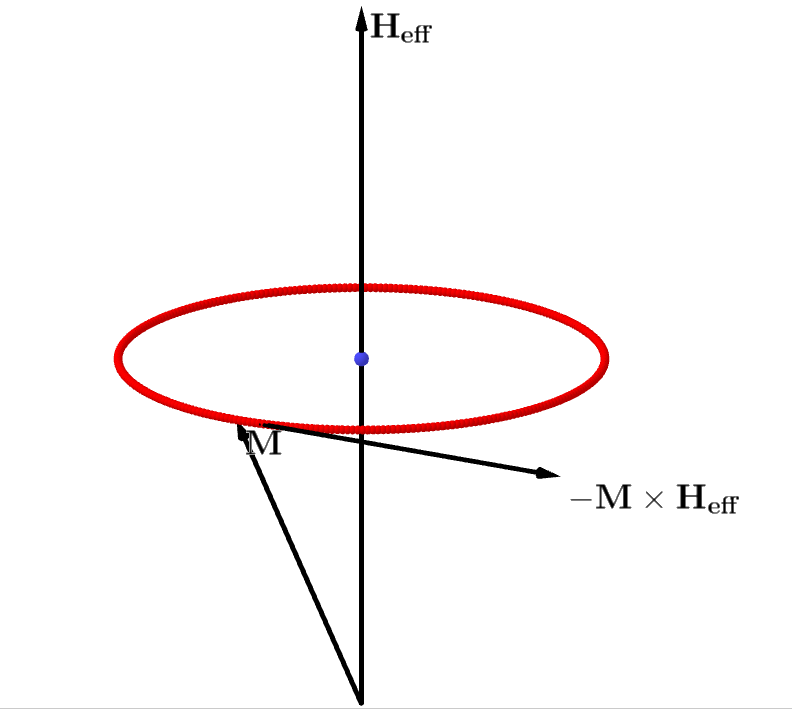
\includegraphics[width=6cm]{fig/precession.png}
				%\caption{fig1}
			\end{minipage}%
		}%
		\subfigure[Damping Precession]{
			\begin{minipage}[t]{0.45\linewidth}
				\centering
				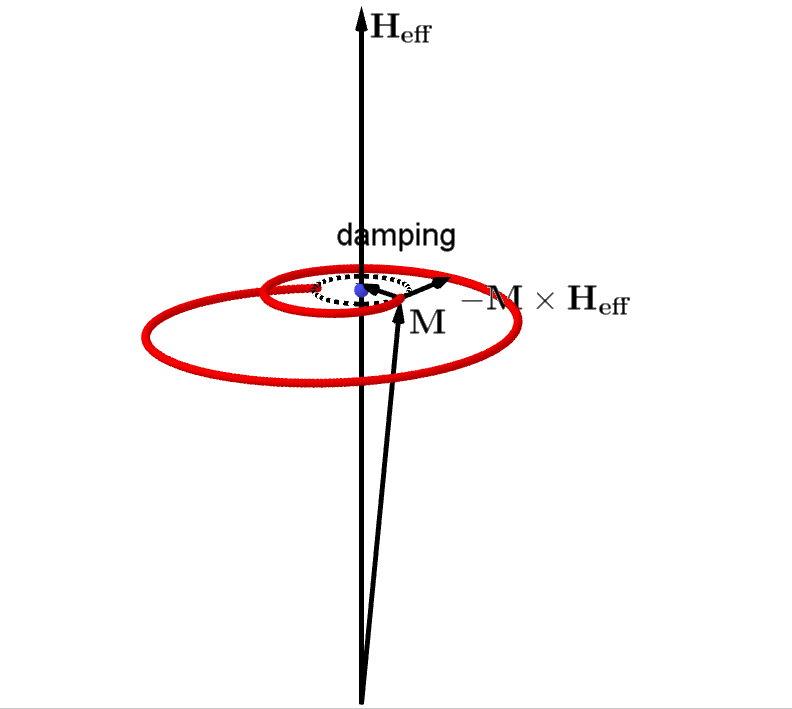
\includegraphics[width=6cm]{fig/precession_damping.png}
				%\caption{fig2}
			\end{minipage}%
		}%
		\caption{拉莫尔进动示意图} \label{img:1.1}
	\end{figure}

	这是一个图片\ref{img:1.1}的引用。
	
	这是一个图片示例:
	
	\begin{figure}[htbp]
		\centering
		\subfigure[Undamping Precession]{
			\begin{minipage}[t]{0.45\linewidth}
				\centering
				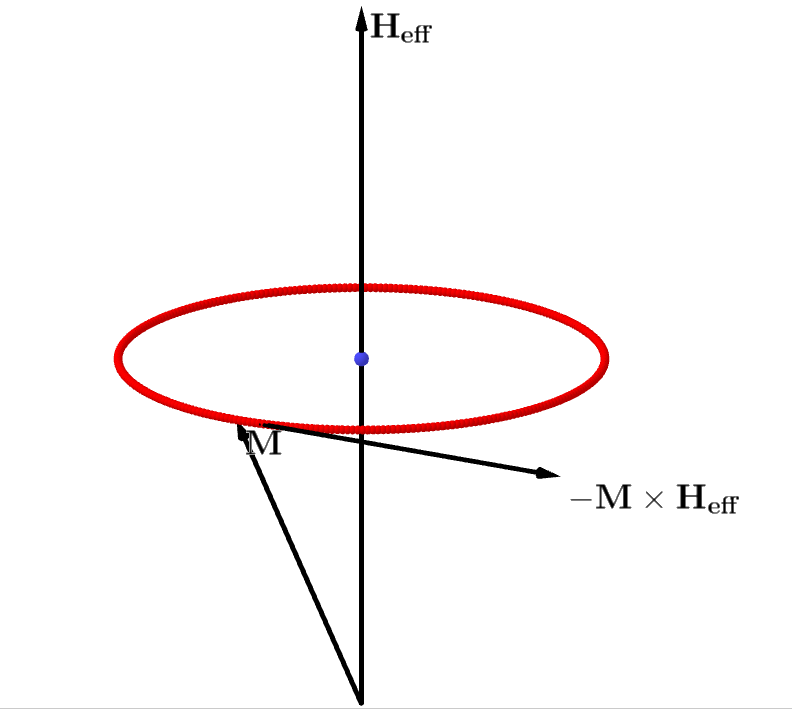
\includegraphics[width=6cm]{fig/precession.png}
				%\caption{fig1}
			\end{minipage}%
		}%
		\subfigure[Damping Precession]{
			\begin{minipage}[t]{0.45\linewidth}
				\centering
				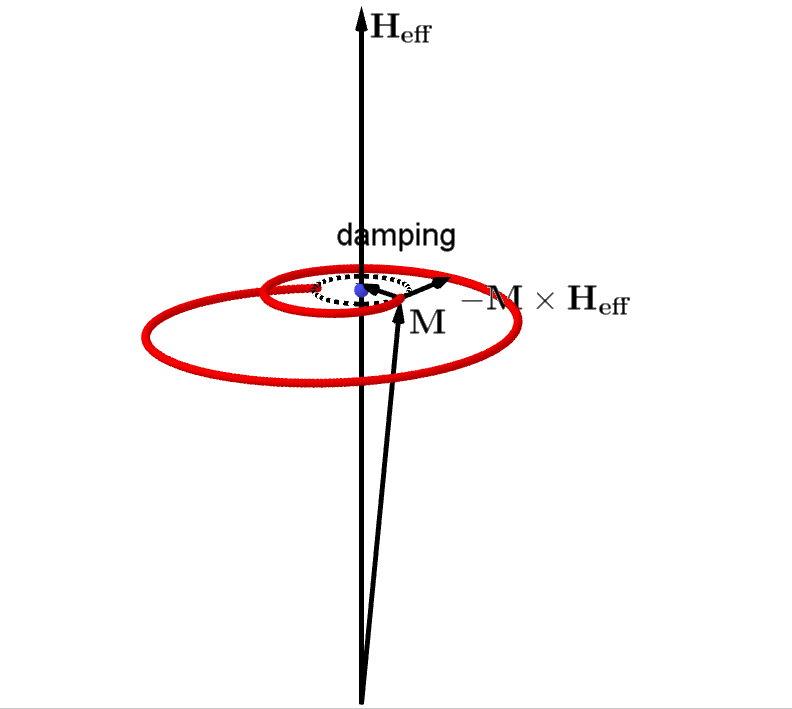
\includegraphics[width=6cm]{fig/precession_damping.png}
				%\caption{fig2}
			\end{minipage}%
		}%
		\caption{拉莫尔进动示意图} \label{img:1.2}
	\end{figure}

	这是一个图片\ref{img:1.2}的引用。
	
	微磁学是磁学的一个分支。其研究对象为介观尺度下铁磁体的磁化过程。该尺度足够大,大到到原子的大小可忽略不计,因此在该尺度下材料的磁化强度矢量是连续的;该尺度又足够小,小到可以看清磁畴的结构,从而可以反映出磁畴间磁矩的过渡状态。微磁学主要解决两类问题:
	
	1)静微磁学:通过最小化磁学能量,得到系统的稳定解;
	
	2)动微磁学:通过解朗道-利夫希兹-吉尔伯特方程式(Landau–Lifshitz–Gilbert, LLG),得到系统的动力学解。
	
	在给定温度$ T_s $下,铁磁体中任意位置处的局部磁化强度矢量等于自发磁化强度$ M_s $即:
	\begin{align}
	|{\bf{M}}({\bf{r}},t)| = {M_s}
	\end{align}	
	
	对于动态系统,一般从系统能量和磁化强度矢量的状态(运动过程)两方面来研究。对于铁磁体,考虑宏观小微观大的区域,即该区域足够小到可以看作一个点,同时又足够大到包含很多基本磁矩。如果忽略磁弹性能、表面各向异能,磁体中的能量可以表述为四种能量之和:各向异相能$ E_{an} $、交换能$ E_{ex} $、静磁能$ E_m $、塞满能$ E_a $。铁磁体的自由能函数可以表示为:
	\begin{align}
		G\left(\mathbf{M}, \mathbf{H}_{\mathrm{a}}\right) &=E_{\mathrm{ex}}+E_{\mathrm{an}}+E_{\mathrm{m}}+G_{\mathrm{a}}= \notag \\  
		&=\int_{\Omega}\left\{A\left[\left(\nabla m_{x}\right)^{2}+\left(\nabla m_{y}\right)^{2}+\left(\nabla m_{z}\right)^{2}\right]+f_{\mathrm{an}}+\right.  \notag \\
		&\left.-\frac{1}{2} \mu_{0} \mathbf{M} \cdot \mathbf{H}_{\mathrm{m}}-\mu_{0} \mathbf{M} \cdot \mathbf{H}_{\mathrm{a}}\right\} d V   \label{eq:1.1}
	\end{align} 
	将上式表示成更加紧凑的形式为:
	\begin{align}
	G\left(\mathbf{M}, \mathbf{H}_{\mathrm{a}}\right)=\int_{\Omega}\left[A(\nabla \mathbf{m})^{2}+f_{\mathrm{an}}+-\frac{1}{2} \mu_{0} \mathbf{M} \cdot \mathbf{H}_{\mathrm{m}}-\mu_{0} \mathbf{M} \cdot \mathbf{H}_{\mathrm{a}}\right] d V \label{eq:1.2}
	\end{align} 
	下面分别说明四种能量的作用:
	
	1)交换相互作用使得周围空间中的磁矩处于平行(在铁磁性材料中)或者反平行(在反铁磁材料中)状态。交换相互作用使得交换能总是处于最小值。
	
	2)各向异性是由于晶格结构产生的特殊的对称性,在没有施加外部磁场情况下,铁磁体的磁化方向趋向于沿着易于磁化的方向,该方向被称为易轴,相应的存在难轴。各向异性使得磁各向异能总是处于最小值。
	
	3)静磁相互作用属于铁磁体内的基本磁矩之间的长距相互作用。铁磁体内的静磁场取决于其中的磁化强度矢量场,静磁场可以通过求解被磁化的介质中的麦克斯韦方程组来得到。静磁相互作用也总使得静磁能处于最小值。
	\begin{align}
	\nabla  \times {{\bf{H}}_{\rm{m}}}{\rm{ = 0}} && \nabla  \cdot {{\bf{H}}_{\rm{m}}}{\rm{ =  - }}\nabla  \cdot {\rm{M}} \label{eq:1.3}
	\end{align}
	
	4)塞满相互作用总使得磁矩平行于外磁场,使得能量最低。这里引入了吉布斯自由能函数,它可以看作受外部场$ {{\bf{H}}_a} $影响,磁矩分布的势能。	
	
	由于四种能量中的任何一个都希望能达到最小值,同时又尽可能小的影响其它三种能量,因此导致了复杂的物理相互作用。
	
	容易知道,磁化强度是单位体积的磁矩,因此,当作用在任何体积元$ dV $里的磁矩$ {\bf{M}}dV $上的力矩为零时,铁磁体处于热力学平衡状态。由磁场$ \bf{H} $引起磁矩$ {\bf{M}}dV $上的力矩可以表示为:
	\begin{align}
	{\bf{T}} = {\mu _0}{\bf{M}}dV \times {\bf{H}}
	\end{align}
	
	如果仅仅考虑外部磁场$ {{\bf{H}}_{\bf{a}}} $作用下的塞曼能,显然,上式中的$ {\bf{H}} $可以表示为$ {{\bf{H}}_{\bf{a}}} $,当考虑所有能量作用的情况下,上式中的$ {\bf{H}} $定义为有效场$ {{\bf{H}}_{{\bf{eff}}}} $,每一个能量项都对有效场有贡献。因此,考虑上述四种能量对应的场,有效场定义为:
	\begin{align}
	{{\bf{H}}_{{\bf{eff}}}} = {{\bf{H}}_{\bf{a}}} + {{\bf{H}}_{\bf{m}}} + {{\bf{H}}_{{\bf{an}}}} + {{\bf{H}}_{{\bf{ex}}}} \label{eq:1.4}
	\end{align}
	
	当磁矩受到的力矩为零时,可以得到系统处于平衡状态时的布朗方程:
	\begin{align}
	{\bf{M}} \times {{\bf{H}}_{{\bf{eff}}}} = 0  \label{eq:1.5}
	\end{align}
	
	当然,考虑到磁化强度最终是要处于稳定的状态,这个状态的显著标志就是自由能最小,为此对自由能关于磁化强度求变分,令其值为0,亦可以得到上述的布朗方程以及有效场的准确表达式。
	
	布朗方程描述了系统处于平衡状态的情况,此时磁化强度矢量$ {\bf{M}} $的方向与有效场$ {{\bf{H}}_{{\bf{eff}}}} $的方向相同。当两者方向不一致时就会出现拉莫尔进动现象,即系统处于非平衡状态$ {\bf{M}} \times {{\bf{H}}_{{\bf{eff}}}} \ne 0 $时,系统状态将会随时间变化,由于阻尼的存在,拉莫尔进动的半径逐渐衰减,最终磁化强度矢量$ {\bf{M}} $的方向与有效场$ {{\bf{H}}_{{\bf{eff}}}} $的方向相同,系统重新达到稳定状态。Landau-Lifshitz(LL)方程即描述了该过程:
	\begin{align}
	\frac{\partial \mathbf{M}}{\partial t}=-\gamma_L \mathbf{M} \times \mathbf{H}_{\mathrm{eff}}-\frac{\lambda}{M_{s}} \mathbf{M} \times\left(\mathbf{M} \times \mathbf{H}_{\mathrm{eff}}\right) \label{eq:1.7}
	\end{align}	
	
	其中$ \gamma_L $表示Landau-Lifshitz旋磁比,$ \lambda  = \gamma \alpha $,$ \alpha $表示阻尼系数或者称为耗散常数。
	当忽略耗散过程,即$ \alpha=0 $时.相应的LL方程形式如下:
	\begin{align}
	\frac{{\partial {\bf{{\rm {M}}(r,}}t{\bf{)}}}}{{\partial t}} =  - \gamma {\bf{M}} \times {{\bf{H}}_{{\bf{eff}}}}  \label{eq:1.6}
	\end{align}
	上述方程两侧同点乘$ \bf{M} $,可以发现$ \partial |{\bf{{\rm M}}}{|^2}/\partial t = 0 $,即LL方程是守恒的。
	
	Gilbert从另一个角度出发,建立了描述磁化动力学的Landau-Lifshitz-Gilbert(LLG)方程:
	\begin{align}
	\frac{\partial \mathbf{M}}{\partial t}=-\gamma_G \mathbf{M} \times \mathbf{H}_{\mathrm{eff}}+\frac{\alpha}{M_{s}} \mathbf{M} \times \frac{\partial \mathbf{M}}{\partial t} \label{eq:1.8}
	\end{align}
	
	实际上LL方程与LLG方程在数学上是等价的($ {\gamma _L} = {\gamma _G}/(1 + {\alpha ^2}) $),但是考虑到耗散项形式的不同,LL方程与LLG方程有着本质的区别。
	
	\section{磁化强度的翻转过程}
	
	
	
	
	\chapter{非线性磁化动力学数值积分}
	\section{数学基础:中点法则数值方法}
	这是一个行间公式:
	\begin{align}
	{\bf{m \times }}{{\bf{h}}_{{\bf{eff}}}} = 0  \label{eq:2.1}
	\end{align}
	
	这是公式\ref{eq:2.1}的交叉引用。
	
		这是一个图片示例:
	
	\begin{figure}[htbp]
		\centering
		\subfigure[Undamping Precession]{
			\begin{minipage}[t]{0.45\linewidth}
				\centering
				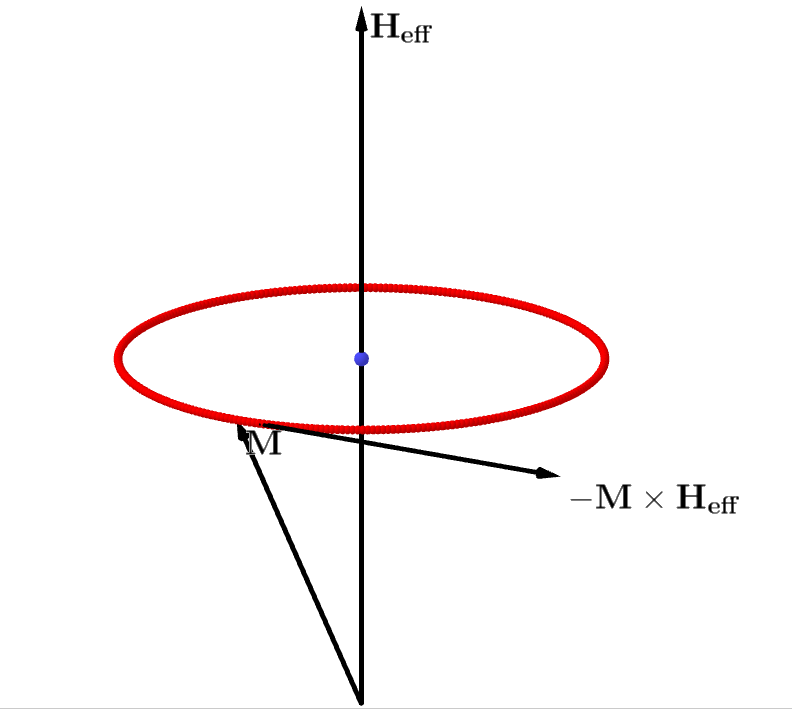
\includegraphics[width=6cm]{fig/precession.png}
				%\caption{fig1}
			\end{minipage}%
		}%
		\subfigure[Damping Precession]{
			\begin{minipage}[t]{0.45\linewidth}
				\centering
				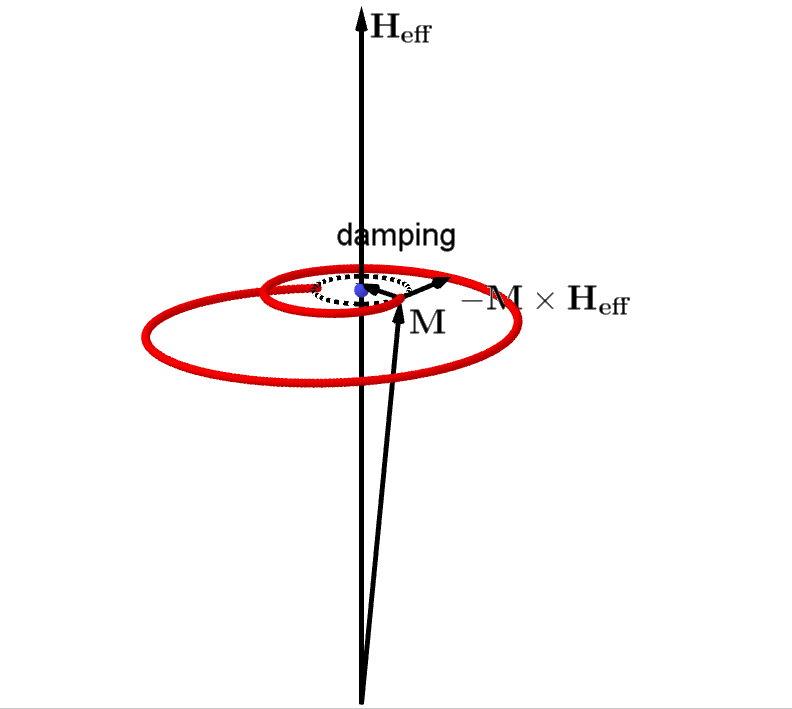
\includegraphics[width=6cm]{fig/precession_damping.png}
				%\caption{fig2}
			\end{minipage}%
		}%
		\caption{拉莫尔进动示意图} \label{img:2.1}
	\end{figure}
	
	这是一个图片\ref{img:2.1}的引用。
	
	
	\section{中点差分法离散形式的LLG方程}
	
	
	
	
	\chapter{仿真分析}
	\section{OOMMF简介}
	\section{问题描述}
	\section{结果展示与分析}
	
	这是一个参考文献引用\cite{mayergoyz2009nonlinear}
	
	
	
	
	
	\label{unknown}